% !TeX spellcheck = en_US
\documentclass{article}
\usepackage{graphicx}
\usepackage{fancybox}
\usepackage{tikz}
\usepackage{amssymb}
\usepackage{algorithm}
\usepackage{amsmath}
\usepackage{algorithmicx}
\usepackage{algpseudocode}
\usepackage{graphicx}
\usepackage{hyperref}
\usepackage{enumitem}
\usepackage{fancybox}
\usepackage{tikz}
\usepackage{caption}

\captionsetup{labelfont={color=black,bf}}


\makeatletter
\def\BState{\State\hskip-\ALG@thistlm}
\makeatother

\algdef{SE}[DOWHILE]{Do}{doWhile}{\algorithmicdo}[1]{\algorithmicwhile\ #1}%

\title{Homework 05: Sorting (Part 2)}
\date{\today}
\author{Roberto Corti}

\begin{document}
	\maketitle
	
	\section*{Exercise 1,2}
	\textbf{Generalize the SELECT algorithm to deal also with repeated values and prove that it still belongs to $O(n)$. Download the latest version of the code from}
	\begin{center}
		\url{https://github.com/albertocasagrande/AD_sorting}
	\end{center}
	\textbf{and} 
	\begin{itemize}
		\item \textbf{Implement the SELECT algorithm of Ex. 1.}
		\item \textbf{Implement a variant of the QUICK SORT algorithm using above mentioned SELECT to identify the best pivot for partitioning.}
		\item \textbf{Draw a curve to represent the relation between the input size and the execution-time of the two variants of QUICK SORT (i.e, those of Ex. 2 and Ex. 1 31/3/2020) and discuss about their complexities.}
	\end{itemize}

	\noindent The new version of SELECT that deals with repeated values described in the previous section is implemented inside the file \texttt{select.c} and \texttt{quick\_sort.c} for the tri-partition implementation.\\
	Once applied this algorithm, I implemented a variant of QUICK SORT using the SELECT method in order to choose the best pivot:
	
		\begin{algorithm}
		\texttt{Quick-Sort Select(A, left, right):} \label{ex2}
		\begin{algorithmic}
			\While {$\mathtt{left \space \leq \space right}$}
			\State \texttt{pivot} $\gets$ \texttt{select\_pivot(A, left, right)}
			\State \texttt{Quick-Sort  Select(A, left, k.first)}
			\State \texttt{left} $\gets$ \texttt{k.second+1}
			\EndWhile
			
		\end{algorithmic}
	\end{algorithm}

	\newpage
	
	\noindent The results, compared with the classic version of QUICK SORT, are represented in the following plot.
	
	\begin{figure}[h]
		\centering
		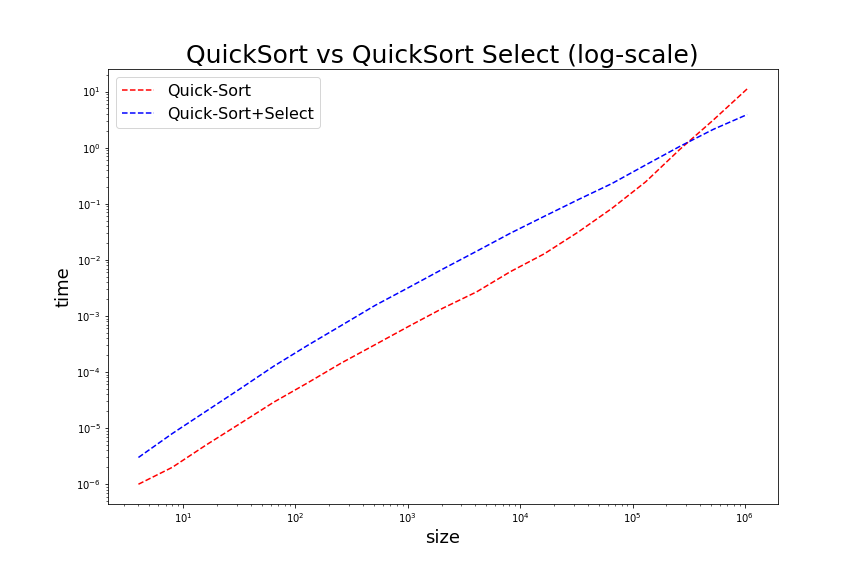
\includegraphics[width=.8\textwidth]{../plot/quicksort.png}  
		\caption{Benchmark of the \texttt{quick\_sort} method compared to its version when the \texttt{select} algorithm is involved in the selection of the pivot.}
		\label{plot}
	\end{figure}
	
	\noindent As it can be observed, the classic QUICK SORT has better performances on small list sizes. However, for big arrays the cost of partitioning becomes relevant and in those cases QUICK-SORT SELECT results to be more efficient.
	
	
	\section*{Exercise 3}
	\textbf{(Ex. 9.3-1 in [1]) In the algorithm SELECT, the input elements are divided into chunks of 5. Will the algorithm work in linear time if they are divided into chunks of 7? What about chunks of 3?} \\
	
	\noindent In the case of having divided into chunks of 7, as we did at lesson, we can get a lower bound on the number of elements that are greater than the median-of-median (say $\hat{m}$), that is 
	$$
	4 \bigg(\bigg\lceil \frac{1}{2} \Big\lceil \frac{n}{7} \Big\rceil \bigg\rceil
	- 2 \bigg) \ge \frac{2n}{7} - 8.
	$$
	Then, the upper bound for the number of elements smaller or equal to $\hat{m}$ is 
	$$
	n-\Big(\frac{2n}{7} - 8\Big) = \frac{5n}{7} +8,
	$$
	and this leads to the following recurrence:
	$$
	T_S(n)=T_S(\lceil n/7 \rceil) + T_S(5n/7 + 8) + \Theta(n).
	$$
	Selecting $cn$ and $c'n$ as representatives of $O(n)$ and $\Theta(n)$ and assuming that $T_S(m) \leq cm$ $\forall m < n$ 
	\begin{align}
	\nonumber
	T(n) & \le c\lceil n/7 \rceil + c(5n/7 + 8) + c'n \\
	\nonumber
	& \le cn/7 + c + 5cn/7 + 8c + c'n \\
	\nonumber
	& = 6cn/7 + 9c + c'n \\
	\nonumber
	& = cn + (-cn/7 + 9c + c'n). 
	\end{align}
	which is at most $cn$ if $ (-cn/7 + 9c + c'n) \le 0 $. This is equivalent to $ c \ge \frac{7c'n}{n - 63}$ and picking $n\geq 126$ and $c\geq 14c'$, we get $T_S(n) \leq cn$ and $T_S(n) \in O(n)$.
	\\
	
	If we divide in groups of 3, the number of elements that are greater than the median-of-medians $\hat{m}$ is:
	
	$$
	2 \bigg(\bigg\lceil \frac{1}{2} \Big\lceil \frac{n}{3} \Big\rceil \bigg\rceil
	- 2 \bigg) \ge \frac{n}{3} - 4,
	$$
	so the upper bound for the number of elements smaller or equal to $\hat{m}$ is 
	$$
	n-\Big(\frac{n}{3} - 4\Big) = \frac{2n}{3} +4.
	$$
	The recurrence is thus 
	$$
	T(n) = T(\lceil n/3 \rceil) + T(2n/3 + 4) + \Theta(n).
	$$
	We guess that $T(n)>cn$ and bounding the non-recursive term with $c'n$:
	\begin{align}
	\nonumber
	T(n) & > c\lceil n/3 \rceil + c(2n/3 + 2) + an \\
	\nonumber
	& > cn/3 + c + 2cn/3 + 2c + an \\
	\nonumber
	& = cn + 3c + an \\
	\nonumber
	& > cn ,
	\end{align}
	which holds for any $c>0$.
	\newpage
	\section*{Exercise 4}
	\textbf{(Ex. 9.3-5 in [1]) Suppose that you have a “black-box” worst-case linear-time subroutine to get the position in A of the value that would be in position $n/2$ if A was sorted. Give a simple, linear-time algorithm that
	solves the selection problem for an arbitrary position i.}\\

	\noindent Let $A$ be the array and denote by $i$ the arbitrary position. The black-box subroutine if applied to $A$ returns the $n/2$ element. If $i=n/2$ the problem is solved. Otherwise, we can partition $A$ into $A_1$, $A_2$ those elements are respectively lower and greater than $A[n/2]$. If $i<n/2$, we will call recursively the algorithm on $A_1$ by searching its $i$th element. If $i>n/2$, the recursive call will be done on $A_2$ by looking for the element $i-n/2$.
	
		\begin{algorithm}
		\texttt{SELECTION(A,i):} 
		\begin{algorithmic}
			\State \texttt{BLACK-BOX(A)} 
			\State \textbf{if} \texttt{i=n/2} \texttt{return A[n/2]}
			\State \texttt{DIVIDE(A)}
			\State \textbf{if} \texttt{i<n/2} \texttt{return SELECTION(A1,i)}
			\State \textbf{else} \texttt{return SELECTION(A2,i-n/2)}
			
		\end{algorithmic}
	\end{algorithm}
	
	The cost of using the black-box subroutine is $O(n)$ and the cost of dividing the array is $O(n)$ too. Let $T(n)$ be the cost of the algorithm described above. Then,
	\begin{align}
	\nonumber
	T(n) & \leq cn + T(n/2) \\
	\nonumber
	& = c(n+n/2+n/4+...+T(1))\\
	\nonumber
	& \leq 2cn \in O(n). 
	\end{align}
	
	
	\section*{Exercise 5}
	\textbf{Solve the following recursive equations by using both the recursion tree and the substitution method:}
	\begin{enumerate}
		\item $T_1(n) = 2 \cdot T_1(n/2) + O(n)$
		\item $T_2(n) = 2 \cdot T_2 \left(  \lceil n/2 \rceil \right)  + T_2 \left( \lfloor n/2 \rfloor \right) + \Theta(1)$
		\item $T_3(n) = 3 \cdot T_3(n/2) + O(n)$
		\item $T_4(n) = 7 \cdot T_4(n/2) + \Theta(n^2)$
	\end{enumerate}
	
	\noindent 1. \textit{Recursion Tree}: \\ The recurrent equation $T_1(n) = 2 \cdot T_1(n/2) + O(n)$  gives rise to the following recursive tree \\

	\begin{figure}[h]
		\begin{center}
			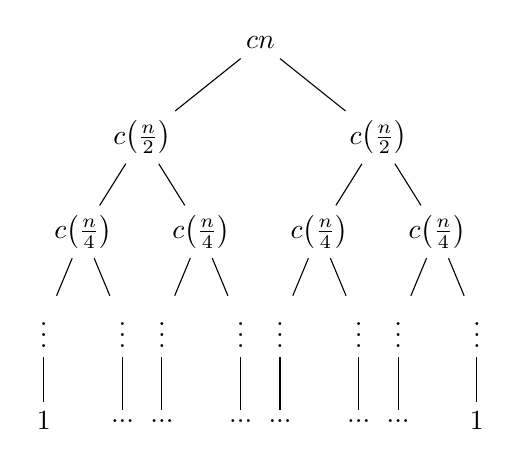
\begin{tikzpicture}[level distance=1.2cm,
			level 1/.style={sibling distance=3cm},
			level 2/.style={sibling distance=1.5cm},
			level 3/.style={sibling distance=1cm},
			level 4/.style={sibling distance=0.4cm},
			level 5/.style={sibling distance=0.2cm}]
			\node {$cn$}
			child {node {$c\big(\frac{n}{2}\big)$}
				child {node {$c\big(\frac{n}{4}\big)$}
					child {
						node {$\vdots$}
						child {node {$1$} 
						}
					}
					child {
						node {$\vdots$}
						child {node{$...$} 
						}
					}   
				}
				child {node {$c\big(\frac{n}{4}\big)$}
					child {
						node {$\vdots$}
						child {node {$...$} 
						}
					}
					child {
						node {$\vdots$}
						child {node{$...$} 
						}
					}   
				}
			}
			child {node {$c\big(\frac{n}{2}\big)$}
				child {node {$c\big(\frac{n}{4}\big)$}
					child {
						node {$\vdots$}
						child {node {$...$} 
						}
					}
					child {
						node {$\vdots$}
						child {node{$...$} 
						}
					}   
				}
				child {node {$c\big(\frac{n}{4}\big)$}
					child {
						node {$\vdots$}
						child {node {$...$} 
						}
					}
					child {
						node {$\vdots$}
						child {node{$1$} 
						}
					}   
				}
			};
			\end{tikzpicture}
			\label{recursion_tree_1}
		\end{center}
	\end{figure}
	\noindent Summing up all the contribution given at each tree level we end up with
	
	\begin{eqnarray}
	\nonumber
	T_1(n) &=& \sum_{i=0}^{\log_2 n -1 } cn + \Theta(n), \\
	\nonumber
	&=& cn\log_2 n + \Theta(n)  \in O(n\log_2n), 
	\nonumber 
	\end{eqnarray} 
	\noindent thus $T_1(n) \in O(n) ~~~ \square$\\
	
	\noindent \textit{Substitution Method}:
	\begin{itemize}
		\item \textbf{Guess}: $T_1(n) \in O(n\log_2 n)$, 
		\item \textbf{Inductive hypothesis}: $\forall m < n, ~  T_1(m) \leq cm\log_2 m$ 
	\end{itemize} 
	In order to prove the guess for $n$ consider $c'n$ as a representative of $O(n)$. Then, considering the equation and using the inductive hypothesis,
	\begin{eqnarray}
	\nonumber
	T_1(n) &=& 2 T_1 (n/2) + c'n,\\
	\nonumber
	&\leq& 2 c \frac{n}{2} \log_2\frac{n}{2} + c'n,\\
	\nonumber
	 &\leq& cn\log_2 n -cn + c'n \leq cn\log_2 n \Leftrightarrow c \geq c' ~~~ \square
	 \nonumber 
	\end{eqnarray} 
	
	\noindent 2.\textit{Recursion Tree} \\
	The recurrent equation $T_2(n) = 2 \cdot T_2 \left(  \lceil n/2 \rceil \right)  + T_2 \left( \lfloor n/2 \rfloor \right) + \Theta(1)$ give rise to an unbalanced tree in which the left-most branch involves only ceiling operation, while the right-most branch will involve only floor operations.
	\newpage
	\begin{figure}[ht]
		\begin{center}
			\begin{tikzpicture}[level distance=1.2cm,
			level 1/.style={sibling distance=3cm},
			level 2/.style={sibling distance=1.5cm},
			level 3/.style={sibling distance=1cm},
			level 4/.style={sibling distance=1cm},
			level 5/.style={sibling distance=1.cm}
			level 6/.style={sibling distance=0.2cm}]
			\node {$n$}
			child {node {$\lceil \frac{n}{2} \rceil $}
				child {node {$\big \lceil \frac{\lceil n/2 \rceil}{2} \big \rceil $}
					child {
						node {$\dots$}
						child { node{$...$} 
								child{ {node{$1$}}
								}
								child[missing] {node {}}
						  	}
						child[missing] {node {}}
					}
					child[missing] {node {}}
				}
				child {node {$\dots$}
					child {
						node {$\dots$}
					}
					child {
						node {$\dots$}
					}
				}
			}
			child {node {$ \lfloor \frac{n}{2} \rfloor $}
				child {node {$\dots$}
					child {
						node {$\dots$}
					}
					child {
						node {$\dots$}
					}
				}
				child {node {$\big \lfloor \frac{\lfloor n/2 \rfloor}{2} \big \rfloor $}
					child {
						node {$\dots$}
					}
					child {
						node {$\dots$}
						child[missing] {node {}}
						child {node{$1$} 
						}
					}   
				}
			};
			\end{tikzpicture}
			\label{recursion_tree_2}
		\end{center}
	\end{figure}
	\noindent The height of the left most branch is at most $\log (2n)$ since $\forall n$ there exists a power of two between the interval $[n, 2n]$ and in case of $n$ equal to this power we have the maximum height of this branch. For what concerns the right most branch, we look for the closer power of two before $n$ and so the height of this branch will be for sure greater than $\log (n/2)$. Thus, considering $c$ as a representative of $\Theta(1)$ and given these two results we can obtain
	\begin{eqnarray}
	\nonumber
	T_2(n) &\geq& \sum_{i=0}^{\log (n/2)} c 2^i, \\
	\nonumber
	&\geq& c \frac{2^{\log (n/2) + 1} -1 }{2-1},\\
	\nonumber
	&\geq& cn -c \Rightarrow T_2(n) \in \Omega(n),
	\nonumber 
	\end{eqnarray}
	and, at the same time,
	\begin{eqnarray}
	\nonumber
	T_2(n) &\leq& \sum_{i=0}^{\log (2n)} c 2^i, \\
	\nonumber
	&\leq& c (2^{\log 2n + 1}-1),\\
	\nonumber
	&\leq& 4cn -c \Rightarrow T_2(n) \in O(n).
	\nonumber 
	\end{eqnarray}
	Then, putting these two results together, $T_2(n) \in \Theta (n) ~~~ \square$\\
	
	
	\noindent \textit{Substitution Method} \\
	In this particular case our goal is to prove that $T_2(n) \in \Theta(n)$ and in order to achieve this thesis we will demonstrate that $T_2(n) \in O(n)$ and, at the same time, $T_2(n) \in \Omega (n) $. \\	
	\begin{itemize}
		\item \textbf{Guess}: $T_2(n) \in O(n)$,
		\item \textbf{Inductive hypothesis}: $\forall m < n, ~  T_2(m) \leq cm - d$
	\end{itemize}
	In order to prove the guess consider $c'$ as a representative of $\Theta(1)$. Then, considering the recurrent equation and the inductive hypothesis,
	\begin{eqnarray}
	\nonumber
	T_2(n) &=&  T_2 \left(  \lceil n/2 \rceil \right)  + T_2 \left( \lfloor n/2 \rfloor \right) + c',\\
	\nonumber
	&\leq&  c \lceil n/2 \rceil -d + \rfloor n/2 \rfloor - d + c' \\
	\nonumber
	&\leq& cn - d - d + c' \leq cn - d \Leftrightarrow d \geq c' ~~~ \square
	\nonumber 
	\end{eqnarray} 
	
	\begin{itemize}
		\item \textbf{Guess}: $T_2(n) \in \Omega(n)$,
		\item \textbf{Inductive hypothesis}: $\forall m < n, ~  T_2(m) \geq cm$
	\end{itemize}
	Also in this case considering $c'$ as a representative of $\Theta(1)$, the recurrent equation and the inductive hypothesis,
	\begin{eqnarray}
	\nonumber
	T_2(n) &=&  T_2 \left(  \lceil n/2 \rceil \right)  + T_2 \left( \lfloor n/2 \rfloor \right) + c',\\
	\nonumber
	&\geq&  cn + c' \geq cn ~~~ \square
	\nonumber  
	\end{eqnarray} 
	
	\noindent 3.\textit{Recursion Tree} \\ The recurrent equation $T_3(n) = 3 \cdot T_3(n/2) + O(n)$  gives rise to the following recursive tree \\

	\begin{figure}[h]
		
		\begin{center}
			
			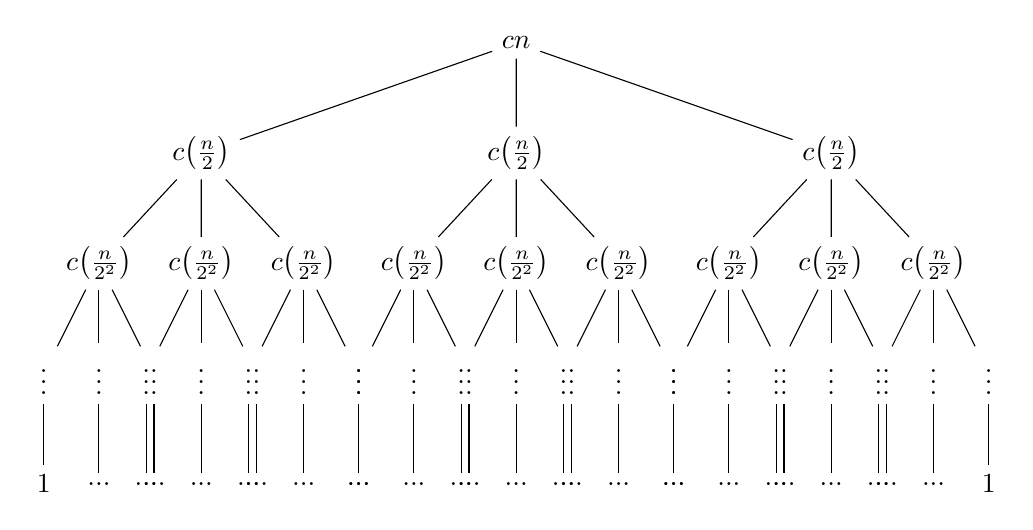
\begin{tikzpicture}[level distance=1.4cm,
			level 1/.style={sibling distance=4cm},
			level 2/.style={sibling distance=1.3cm},
			level 3/.style={sibling distance=0.7cm},
			level 4/.style={sibling distance=0.4cm},
			level 5/.style={sibling distance=0.2cm}]
			\node {$cn$}
			child {node {$c\big(\frac{n}{2}\big)$}
				child {node {$c\big(\frac{n}{2^2}\big)$}
					child {
						node {$\vdots$}
						child {node {$1$} 
						}
					}
					child {
						node {$\vdots$}
						child {node{$...$} 
						}
					}  
					child {
						node {$\vdots$}
						child {node{$...$} 
						}
					}  
				}
				child {node {$c\big(\frac{n}{2^2}\big)$}
					child {
						node {$\vdots$}
						child {node {$...$} 
						}
					}
					child {
						node {$\vdots$}
						child {node{$...$} 
						}
					}  
					child {
						node {$\vdots$}
						child {node{$...$} 
						}
					}  
				}
				child {node {$c\big(\frac{n}{2^2}\big)$}
					child {
						node {$\vdots$}
						child {node {$...$} 
						}
					}
					child {
						node {$\vdots$}
						child {node{$...$} 
						}
					}  
					child {
						node {$\vdots$}
						child {node{$...$} 
						}
					}  
				}
			}
			child {node {$c\big(\frac{n}{2}\big)$}
				child {node {$c\big(\frac{n}{2^2}\big)$}
					child {
						node {$\vdots$}
						child {node {$...$} 
						}
					}
					child {
						node {$\vdots$}
						child {node{$...$} 
						}
					}  
					child {
						node {$\vdots$}
						child {node{$...$} 
						}
					}  
				}
				child {node {$c\big(\frac{n}{2^2}\big)$}
					child {
						node {$\vdots$}
						child {node {$...$} 
						}
					}
					child {
						node {$\vdots$}
						child {node{$...$} 
						}
					}  
					child {
						node {$\vdots$}
						child {node{$...$} 
						}
					}  
				}
				child {node {$c\big(\frac{n}{2^2}\big)$}
					child {
						node {$\vdots$}
						child {node {$...$} 
						}
					}
					child {
						node {$\vdots$}
						child {node{$...$} 
						}
					}  
					child {
						node {$\vdots$}
						child {node{$...$} 
						}
					}  
				}
			}
			child {node {$c\big(\frac{n}{2}\big)$}
				child {node {$c\big(\frac{n}{2^2}\big)$}
					child {
						node {$\vdots$}
						child {node {$...$} 
						}
					}
					child {
						node {$\vdots$}
						child {node{$...$} 
						}
					}  
					child {
						node {$\vdots$}
						child {node{$...$} 
						}
					}  
				}
				child {node {$c\big(\frac{n}{2^2}\big)$}
					child {
						node {$\vdots$}
						child {node {$...$} 
						}
					}
					child {
						node {$\vdots$}
						child {node{$...$} 
						}
					}  
					child {
						node {$\vdots$}
						child {node{$...$} 
						}
					}  
				}
				child {node {$c\big(\frac{n}{2^2}\big)$}
					child {
						node {$\vdots$}
						child {node {$...$} 
						}
					}
					child {
						node {$\vdots$}
						child {node{$...$} 
						}
					}  
					child {
						node {$\vdots$}
						child {node{$1$} 
						}
					}  
				}
			};
			\end{tikzpicture}
			\label{recursion_tree_3}
		\end{center}
		
	\end{figure}
	\noindent Summing up all the contribution given at each tree level we end up with
	
	\begin{eqnarray}
	\nonumber
	T_3(n) &=& cn + \frac{3}{2} cn + ... + \Bigg( \frac{3}{2} \Bigg)^{\log_2 n-1} cn + \Theta(n^{\log_2 3}),\\
	\nonumber
	&=& cn \sum_{i=0}^{\log_2 n - 1} \Bigg( \frac{3}{2} \Bigg)^i + \Theta(n^{\log_2 3}), \\
	\nonumber
	&\leq& \frac{1}{1-3/2}cn + \Theta(n^{\log_2 3}) 
	\end{eqnarray}
	\noindent Thus, taking $c'n^{\log_2 3}$ as a representative of $\Theta(n^{\log_2 3})  $, it holds
	$$ T_3(n) \leq c'n^{\log_2 3} \Rightarrow T_3(n) \in O(n^{\log_2 3}) ~~~ \square$$


	\noindent \textit{Substitution Method}:
	\begin{itemize}
		\item \textbf{Guess}: $T_3(n) \in O(n^{\log_2 3})$,
		\item \textbf{Inductive hypothesis}: $\forall m < n, ~  T_3(m) \leq cm^{\log_2 3} - dm$
	\end{itemize}   
	In order to prove the guess for $n$ consider $c'n$ as a representative of $O(n)$. Then, considering the equation and using the inductive hypothesis,
	\begin{eqnarray}
	\nonumber
	T_3(n) &=& 3 T_3 (n/2) + c'n,\\
	\nonumber
	&\leq& 3 c (n/2)^{\log_2 3} - \frac{3}{2}dn + c'n,\\
	\nonumber
	&\leq& cn^{\log_2 3} - dn - \frac{1}{2} dn + c'n \leq  cn^{\log_2 3}  \Leftrightarrow d \geq 2 c' ~~~ \square
	\nonumber 
	\end{eqnarray} 
	
	\noindent 4.\textit{Recursion Tree} \\ The recurrent equation $T_4(n) = 7 \cdot T_4(n/2) + \Theta(n^2)$  gives rise to the following recursive tree \\

	\begin{figure}[h]
		
		\begin{center}
			
			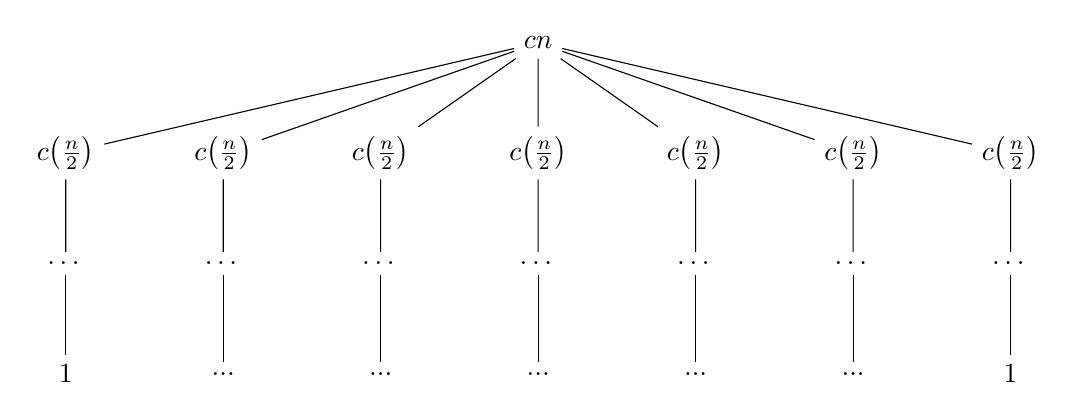
\begin{tikzpicture}[level distance=1.4cm,
			level 1/.style={sibling distance=2cm},
			level 2/.style={sibling distance=2cm},
			level 3/.style={sibling distance=0.7cm},
			level 4/.style={sibling distance=0.4cm},
			level 5/.style={sibling distance=0.2cm}]
			\node {$cn$}
			child {node {$c\big(\frac{n}{2}\big)$}
				child {node {$\dots$}
					child { node{$1$} }
				}
			}
			child {node {$c\big(\frac{n}{2}\big)$}
				child {node {$\dots$}
					child { node{$...$} }
				}
			}
			child {node {$c\big(\frac{n}{2}\big)$}
				child {node {$\dots$}
					child { node{$...$} }
				}
			}
			child {node {$c\big(\frac{n}{2}\big)$}
				child {node {$\dots$}
					child { node{$...$} }
				}
			}
			child {node {$c\big(\frac{n}{2}\big)$}
				child {node {$\dots$}
					child { node{$...$} }
				}
			}
			child {node {$c\big(\frac{n}{2}\big)$}
				child {node {$\dots$}
					child { node{$...$} }
				}
			}
			child {node {$c\big(\frac{n}{2}\big)$}
				child {node {$\dots$}
					child { node{$1$} }
				}
			};
			\end{tikzpicture}
			\label{recursion_tree_4}
		\end{center}
		
	\end{figure}
	\noindent Summing up all the contribution given at each tree level we end up with
	
	\begin{eqnarray}
	\nonumber
	T_3(n) &=& cn^2 + \frac{7}{4} cn + ... + \Bigg( \frac{7}{4} \Bigg)^{\log_2 n-1} cn + \Theta(n^{\log_2 7}),\\
	\nonumber
	&=& cn^2 \sum_{i=0}^{\log_2 n - 1} \Bigg( \frac{7}{4} \Bigg)^i + \Theta(n^{\log_2 7}), \\
	\nonumber
	&\leq& \frac{1}{1-7/4}cn^2 + \Theta(n^{\log_2 7}).
	\end{eqnarray}
	\noindent Thus, taking $c'n^{\log_2 7}$ as a representative of $\Theta(n^{\log_2 7})  $, it holds
	$$ T_3(n) \leq c'n^{\log_2 7} \Rightarrow T_3(n) \in O(n^{\log_2 3}) ~~~ \square$$
	
	
	\noindent \textit{Substitution Method}:
	\begin{itemize}
		\item \textbf{Guess}: $T_4(n) \in O(n^{\log_2 7})$,  
		\item \textbf{Inductive hypothesis}: $\forall m < n, ~  T_4(m) \leq cm^{\log_2 7} - dm^2$ 
	\end{itemize} 
	In order to prove the guess for $n$ consider $c'n^2$ as a representative of $\Theta(n^2)$. Then, considering the equation and using the inductive hypothesis,
	\begin{eqnarray}
	\nonumber
	T_4(n) &=& 7 T_4 (n/2) + c'n^2,\\
	\nonumber
	&\leq& 7 c (n/2)^{\log_2 7} - \frac{7}{4}d + c'n^2,\\
	\nonumber
	&\leq& cn^{\log_2 7} - dn^2 -\frac{3}{4} dn^2 + c'n^2 \leq  cn^{\log_2 7} -dn^2  \Leftrightarrow d \geq \frac{4}{3} c' ~~~ \square
	\nonumber 
	\end{eqnarray} 
\end{document}
